% !TEX program = xelatex

\documentclass{article}
\usepackage{amsfonts,amssymb}
\usepackage{amsmath}
\usepackage{amsthm}
\usepackage[left=1.0cm,right=1.0cm,top=1.3cm,bottom=1.3cm]{geometry}
\usepackage{enumerate}
\usepackage{fancyhdr}
\usepackage{ctex}
\usepackage{xpatch}
\usepackage{graphicx} %插入图片的宏包
\usepackage{float} %设置图片浮动位置的宏包
\usepackage{subfigure} %插入多图时用子图显示的宏包
\usepackage{listings}
\usepackage{color}
\usepackage{amssymb,mathrsfs,amsmath}
\usepackage{bbding}
\usepackage{mathrsfs}

\definecolor{dkgreen}{rgb}{0,0.6,0}
\definecolor{gray}{rgb}{0.5,0.5,0.5}
\definecolor{mauve}{rgb}{0.58,0,0.82}

\lstset{frame=tb,
  language=Python,
  aboveskip=3mm,
  belowskip=3mm,
  showstringspaces=false,
  columns=flexible,
  basicstyle={\small\ttfamily},
  numbers=none,
  numberstyle=\tiny\color{gray},
  keywordstyle=\color{blue},
  commentstyle=\color{dkgreen},
  stringstyle=\color{mauve},
  breaklines=true,
  breakatwhitespace=true,
  tabsize=3
}


\newtheoremstyle{break}
    {\topsep}{\topsep}%
    {\itshape}{}%
    {\bfseries}{}%
    {\newline}{}%
\theoremstyle{break}
\newtheorem*{solution*}{\textbf{Solution:} }
%\newtheorem*{proof*}{\textbf{Proof:}}
\makeatletter

\AtBeginDocument{\xpatchcmd{\@thm}{\thm@headpunct{.}}{\thm@headpunct{}}{}{}}
\makeatother

\pagestyle{fancy} 
\lhead{Name}
\chead{\textbf{Discrete Mathematics:  Homework 10}}
\rhead{2020.5.14}
\renewcommand{\baselinestretch}{1.5}

\title{Discrete Mathematics:  Homework 10}
\author{Name  \quad  \quad ID: Number}
\date{2020.5.14}


\begin{document}
\maketitle
\begin{enumerate}
\item How many was to reaarange the letters of the word  "lexicographic" ?
\begin{solution*}
For the 13 letters, we can have $P_{13}^{1}$ ways to reaarange.\\
For the letter 'i' and 'c', which appears twice as the same letter, we devided by $P_{2}^{1}$  \\
The arrangement doesn't count in itself, so the answer is, \\
$ \frac  {P_{13}^{13} }{P_{2}^{1} P_{2}^{1}} -1 = 1556755119$
\end{solution*}
 \vspace{10mm}
\item How many bit strings are there of length 10, not containing 2 consectivezero's and not starting or ending in 111?
\begin{solution*}
        For the first 3 digits: we have $2^3-1$ situations.\\
        For the rest 7 digits, we have:\\
        $a_1= 1$, $b_1 = 1$, $a_{n+1} = a_n + b_n$, $b_{n+1} = a_n$,\\
        so, we have,\\
        \begin{center}
                \begin{tabular}{|c|c|c|}
                        \hline
                        i & $a_i$ & $b_i$\\
                        \hline
                        1 & 1 & 1 \\
                        \hline
                        2 & 2 & 1 \\
                        \hline
                        3 & 3 & 2 \\
                        \hline
                        4 & 5 & 3 \\
                        \hline
                        5 & 8 & 5 \\
                        \hline
                        6 & 13 & 8 \\
                        \hline 
                        7 & 21 & 13 \\
                        \hline 
                        8 & 34 & 21 \\
                        \hline
                        9 & 55 & 34 \\
                        \hline 
                        10 & 89 & 55 \\
                        \hline
                        \end{tabular}
        \end{center}
        so, the answer is $xxxxx - 111xxxx - xxxx111 + 111xxxx111$\\
        so, the answer is $(a_{10 }+ b_{10 })- (a_7 + b_7) -(a_8)+(a_4+b_4)= 84$
\end{solution*}
\newpage
\item Consider permuatations of the set $ \{1,2,3,4,5,6\}$ , how many permuatationscome after $α= 245136$ in lexicgraphic order?
\begin{solution*}
        $4 \cdot  P_{5}^{5} + 2 \cdot  P_4^4 + P_3^3 + 2 \cdot P_2^2 + 1 = 539$
\end{solution*}
\vspace{10mm}
\item Suppose we have a reguar octahedron with side lengths equal to $\sqrt{2}$.  Given 28 points in the octahedron, prove that there is a collection of 4 points such that thedistance between any two in the collection is at most 2.
\begin{proof}
        \leavevmode\\
        \begin{figure}[H]
                \centering
                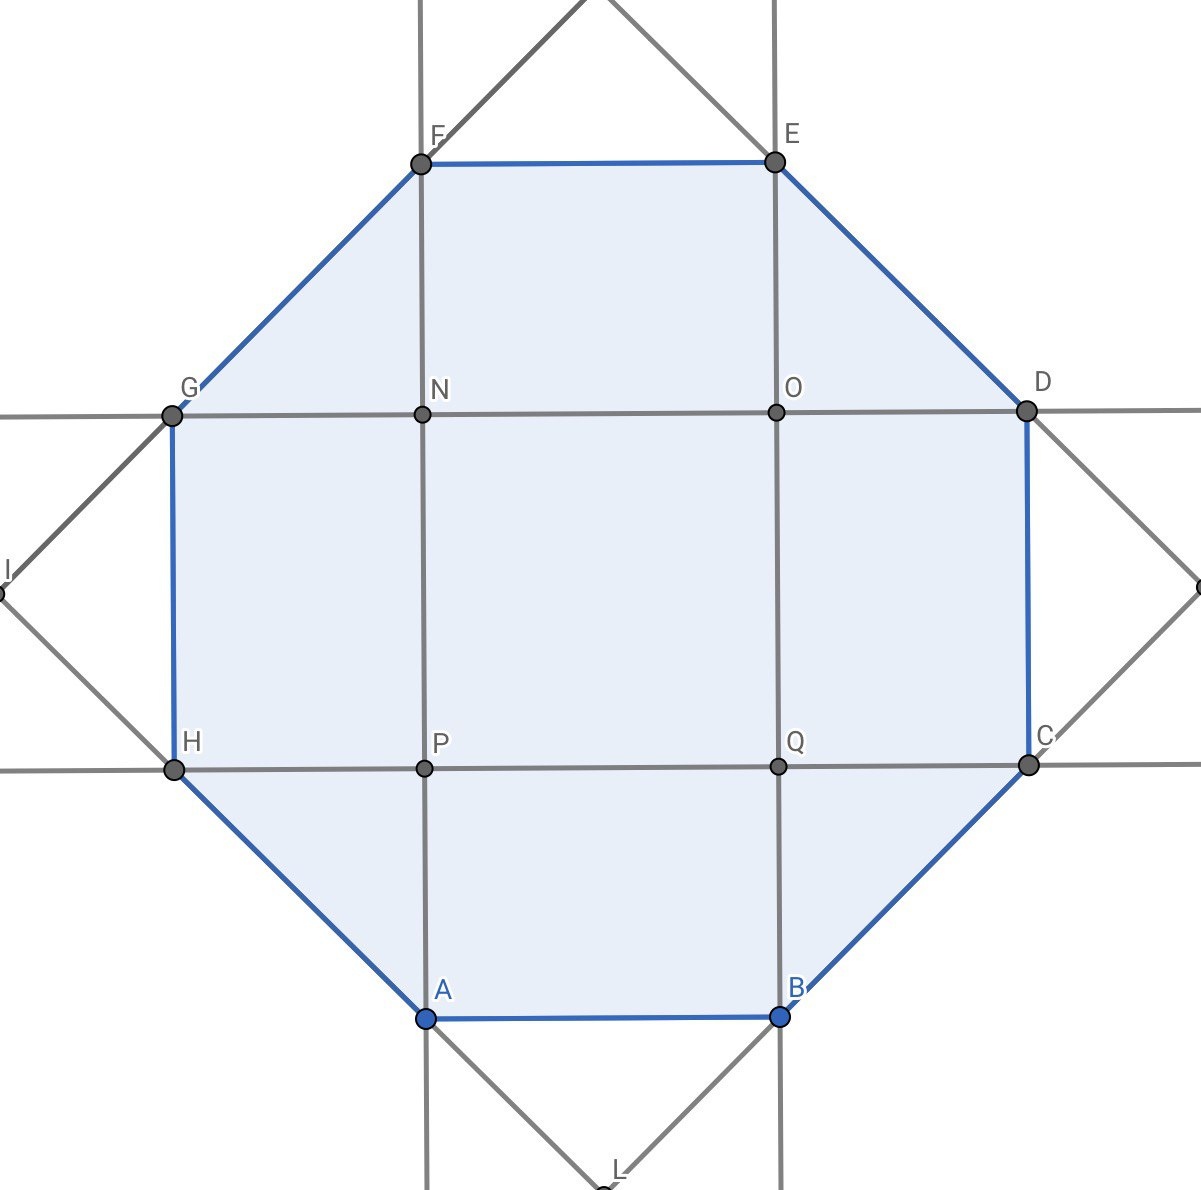
\includegraphics[scale=0.1]{1.jpg}
        \end{figure}
        By the pigeonhole theorem, at least 1 block can have more than $\lfloor \frac{28}{9} +1  \rfloor = 4 $ points.\\
        For the biggest block, the distance between two points can't be larger than 2.\\
        so, there is a collection of 4 points such that thedistance between any two in the collection is at most 2.
\end{proof}
\vspace{10mm}
\item Consider  a  finite  set $A=\{1,2,3,...,m\}$.   Recall  that $P(A)$  is  the  set of  subsets  of $A$ with $|P(A)|=  2^m$.   Count  the  number  of  functions $\tau: P(A)\rightarrow \{0,1,...,m\}$ satisfying
\begin{enumerate}
        \item For any non-empy subset $B$, $\tau(B)>0$.
        \item  For any subsets C and D: $\tau (C \cup D) = \tau(C\cap D) +\tau ((C\cup D) \setminus (C\cap D)).$
\end{enumerate}
\begin{solution*}
        Suppose $C \cap D = \emptyset $, than $\tau (C \cup D) = \tau(\emptyset) +\tau ((C\cup D) \setminus (\emptyset)) = \tau(\emptyset)  + \tau (C\cup D)$\\
        so we have, $\tau(\emptyset) = 0$
        so the rest elements of $P(A)$, which is $2^m - 1$ can maps to the rest $m$ elements.\\
        And $\tau (C \cup D) = \tau(C\cap D) +\tau ((C\cup D) \setminus (C\cap D))$, so the map is "increasing" or "linear"\\
       Suppose $x \in P(A) = a$ ,$y \in P(A) = b$,$x \in P(A) = z$
       $\tau (x + y) = \tau(x) + \tau(y) = a + b$\\
       and $1 \leq a+b \leq m$\\
       $|P(A)| = |\tau|P(A)|$
        so there are only 1 function,\\
\end{solution*}
\newpage
\item Suppose a person delivers packages to a street (the street only has houseson one side,  on the other side is a large building,  which does not receive packages).One day, the person delivers the packages and the two following conditions occur
\begin{enumerate}
        \item There is no n consecutive houses with no packages for n $\geq$ 2
        \item There are no m consecutive houses with packages for m$\geq$3
\end{enumerate}If  the  street  has  14  houses,  and  each  house  receives  at  most  1  package.   how  manypossibile ways to deilver packages on this day?
If  the  street  has  14  houses,  and  each  house  receives  at  most  1  package.   how  many possibile ways to deilver packages on this day?
\end{enumerate}
\begin{solution*}
        $a_1 = 1, b_1 = 2, c_1 = 1$\\
        which represents the i to i+1 digits the number of (0-1) (1-0) (1-1)
        $a_{n+1} = b_{n}, b_{n+1} = a_n+c_n, c_{n+1} = a_n$\\
        so we have,
        \begin{center}
                \begin{tabular}{|c|c|c|c|}
                        \hline
                        i & $a_i$ & $b_i$ & $c_i$\\
                        \hline
                        1 & 1 & 2 & 1 \\
                        \hline
                        2 & 2 & 2 & 1 \\
                        \hline
                        3 & 2 & 3 & 2 \\
                        \hline
                        4 & 3  & 4 & 2 \\
                        \hline
                        5 & 4 & 5 & 3 \\
                        \hline
                        6 & 5 & 7 & 4 \\
                        \hline 
                        7 & 7 & 9 & 5 \\
                        \hline 
                        8 & 9 & 12 & 7 \\
                        \hline
                        9 & 12  & 16 & 9 \\
                        \hline 
                        10 & 16 & 21 & 12 \\
                        \hline
                        11 & 21 & 28 & 16 \\
                        \hline
                        12 & 28 & 37 & 21 \\
                        \hline
                        \end{tabular}
        \end{center}
        so, $a_12 + b_12 + c_12 = 86$ possibile ways to deilver packages on this day.
\end{solution*}
\end{document}